%!TeX root = ../main.tex
\section{Esparcimiento, extinción y absorción}

En la sección anterior, se estudió cómo se relaciona el campo eléctrico que incide en una partícula arbitraria con el campo eléctrico esparcido por esta, dando como resultado la relación de la Ec. \eqref{eq:MEsparcimientoGral}. En esta sección, se estudia el balance de energía al presentarse el fenómeno de esparcimiento.

Supóngase un haz de luz cruza por un medio donde se encuentran partículas arbitrarias (ver Fig. \ref{fig:EnergiaDetector}) y que la energía medida por un detector colocado detrás de las partículas  es $U$. En el caso donde no hubiera partículas, la energía que mediría el detector sería $U_0$ , con $U_0 > U$.  La diferencia de energía $U_0-U$ entre ambos casos es atribuida tanto a la absorción de las partículas (conversión de la energía EM en otras formas de energía, como calor), como al esparcimiento de la luz en direcciones distintas a la posición del detector. Al efecto en conjunto de la absorción y del esparcimiento se denomina extinción.

	\begin{figure}[h!]\centering
%	\tdplotsetmaincoords{60}{110}
%	\pgfmathsetmacro{\rvec}{1. 3}
%	\pgfmathsetmacro{\thetavec}{30}
%	\pgfmathsetmacro{\varphivec}{60}
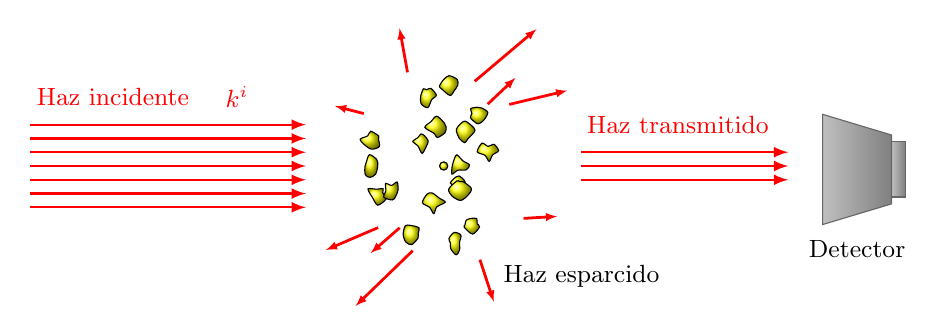
\begin{tikzpicture}[scale=3.5]
\def\d{.75}

%------- Scatterers cloud
\foreach \i in {0,20,40,60,...,360}{
\pgfmathsetseed{\i}
\draw[ball color=yellow, opacity = 1,scale =.03,rotate = rnd, shift={({10*rnd*cos(\i)},{10*rnd*sin(\i)})}]
	 plot [smooth cycle, samples=8,domain={1:8}]
     (\x*360/8+5*rnd:0.5cm+1cm*rnd) node at (0,0) {};
}
%------ Incident wave
	\foreach \i in {-3,...,3}{
		\draw[thick,red, - latex] (-1.5,\i/20)--(-.5,\i/20);}
	\node at (-1.2,5/20){\small \color{red}Haz incidente};	
	\node at (-.75, 5/20) {\small \color{red}$\vb{k}^i$};
%------ Transmitted wave	
	\foreach \i in {-1,...,1}{
\draw[thick,red, - latex] (.5,\i/20)--(1.25,\i/20);}
\node at (.85,3/20){\small \color{red}Haz transmitido};	

%------- Detector
\node at ( 1.5, -6/20){\small Detector};
\begin{scope}[scale  = .25, shift = {(3.5,-2.3)}, rotate = 90, shift = {(-.25,-5)}]
\shade[left color=gray!50!white,right color=gray] (1.7,3)
    -- ++(1.6,0) -- ++(-0.3,-1) -- ++(-1,0) -- cycle;% column
  \shade[left color=gray!50!white,right color=gray] (2.1,2)
    -- ++(0.8,0) -- ++(0,-0.2) -- ++(-0.8,0) -- cycle;% column bottom
  \draw[gray!80!black] (1.7,3) -- ++(1.6,0) -- ++(-0.3,-1)
    -- ++(-1,0) -- cycle;%column
  \draw[gray!80!black] (2.1,2) -- ++(0,-0.2) -- ++(0.8,0)
    -- ++(0,0.2);%column bottom
\end{scope}	

%------- Campo esparcido
\node at ( .5, -8/20){\small Haz esparcido};
\begin{scope}[opacity=1, transparency group, scale = .15]
\foreach \s in {-1,1}{
	\draw[- latex, red](0,\s*\d)++(25:\s*1.75)--(35+rand*5:\s*3.5);
	\draw[- latex, red](0,\s*\d)++(35:\s*1.3)--(55+rand*5:\s*2.75);
	\draw[- latex, red](0,\s*\d)++(165:\s*2)--(155+rand*5:\s*3);
	\draw[- latex, red](0,\s*\d)++(120:\s*1.75)--(110+rand*5:\s*3.5);
	\draw[- latex, red](0,\s*\d)++(60:\s*1.5)--(60+rand*5:\s*4);}
\end{scope}

\end{tikzpicture}
%
\caption{Diagrama de la extinción de luz por una nube de partículas esparcidoras. La energía que mide el detector en la ausencia de partículas es $U_0$ sin embargo, al interactuar la luz con las partículas, la lectura de energía es $U$. La energía $U-U_0$  corresponde a la energía que no llega al detector asociada tanto al esparcimiento de luz, como a la absorbida por las partículas; al conjunto de estos fenómenos se le denomina extinción.}\label{fig:EnergiaDetector}
	\end{figure}	
	
Ahora, considérese el caso de una sola partícula (de tamaño  forma arbitraria) inmersa en un medio dispersor e iluminada por una onda plana; debido a la onda plana, la partícula esparce luz.  Para cuantificar la energía esparcida por la partícula, defínase una esfera $A$ de radio $r$ que contenga a la partícula. La energía total  por unidad de tiempo que cruza la superfice de $A$ se calcula como
%
\begin{align}
W_{abs} = -\int_A\vb{S}\cdot \vu{e}_r \dd{a},
\label{eq:Wa}
\end{align}
%
donde el vector de Poyntig  puede descomponerse en tres contribuciones
%
\begin{align}
\vb{S} &= \frac12 \Re[\vb{E}\times\vb{H}^*] = \vb{S}^i + \vb{S}^s + \vb{S}^{ext},
\label{eq:PoyntingContribuciones}\\
\vb{S}^i &= \frac12 \Re[\vb{E}^i\times\vb{H}^{*i}], \\
 \vb{S}^s &= \frac12 \Re[\vb{E}^s\times\vb{H}^{s*}] ,\\
\vb{S}^{ext} &= \frac12 \Re[\vb{E}^i\times\vb{H}^{s*} + \vb{E}^s \times\vb{H}^{i*}],
\label{eq:Sext}
\end{align}
%
siendo $i$, $s$ y $ext$ los subíndices que denotan a los campos EMs incidentes, el esparcidos y el extintos, respectivamente.

Según la Ec \eqref{eq:Wa}, si $W_{abs}>0$ entonces la energía es absorbida dentro de la esfera, y si $W_{abs}<0$ entonces energía es generada en la partícula, aunque a lo largo de este texto se excluye este caso. Al descomponer a $W_{abs}$ en las mismas contribuciones que al  vector de Poynting en la Ec. \eqref{eq:PoyntingContribuciones}, obtenemos que
%
\begin{align}
W_{abs} &= W_i -W_s + W_{ext},
\end{align}
%
con
%
\begin{align}
W_{i} = -\int_A\vb{S}^i\cdot \vu{e}_r \dd{a} = 0,\\
W_s = \int_A\vb{S}^s\cdot \vu{e}_r \dd{a},\\
W_{ext} = -\int_A\vb{S}^{ext}\cdot \vu{e}_r \dd{a},
\end{align}
%
donde $W^i=0$ dado que la partícula se encuentra en un medio no disipativo. Es decir, que la energía extinta por unidad de tiempo es
%
\begin{align}
W_{ext} = W_{abs} + W_s,
\end{align}
%
como se describió al inicio de esta sección.	

Como caso particular, supóngase que la onda plana incidente está polarizada en la dirección $x$, es decir que $\vb{E}^i = E_0\vu{e}_x$, con $E_0$	 la amplitud del campo eléctrico incidente. Empleando la  expresión para el campo eléctrico esparcido $\vb{E}^s$ como función del campo incidente [Ec. \eqref{eq:MEsparcimientoGral}] y empleando la Ec. \eqref{eq:EIncidenteFull}, así como la ley de Faraday-Lenz, los campos EMs esparcidos se escriben como
%
\begin{align}
\vb{E}^s(\vb{r}) &\propto \frac{e^{ik(r-z)}}{-ikr}E_0\vb{X}(\theta,\varphi),
\label{eq:EscaX}\\
\vb{H}^s(\vb{r}) &\propto \frac{e^{ik(r-z)}}{kr\omega\mu}E_0\vu{e}_r\times\vb{X}(\theta,\varphi),
\label{eq:HscaX}
\end{align}
%
con $\vb{X}\cdot\vu{e}_r = 0$ dada por
%
\begin{align}
\vb{X}(\theta,\varphi) = (S_2\cos\varphi + S_3\sin\varphi)\vu{e}_{\parallel}^s + (S_4\cos\varphi + S_1\sin\varphi)\vu{e}_{\perp}^s,
\end{align}
%
donde $S_j = S_j(\theta,\varphi)$.

Para calcular la energía por unidad de tiempo $W_{ext}$ asociada a la extinción que cruza a una superficie esférica $A$ de radio $r$, se emplean las Ecs. \eqref{eq:Sext}, \eqref{eq:EscaX} y \eqref{eq:HscaX}  (\ref{ex:Wext}), dando como resultado que
%	
\begin{align}
W_{ext} &= -\int_{A} \vb{S}^{ext}\cdot\vu{e}_r\dd{a}\notag\\
 &= \frac{kE_0^2}{2\mu\omega}\Re\bigg\{
\frac{e^{-ikr}}{-ikr}
	\int_A e^{ikz} (\vu{e}_x\cdot\vb{X}^*)\dd{a}\notag\\
&\qquad\qquad+\frac{e^{ikr}}{ikr}
	\int_A e^{-ikz}(\vb{X}\cdot\vu{e}_x)\cos\theta\dd{a}\notag\\
&\qquad\qquad-\frac{e^{ikr}}{ikr}
	\int_A e^{-ikz}(\vb{X}\cdot\vu{e}_z)\sin\theta\cos\varphi\dd{a}
	\bigg\},
	\label{eq:WextX}
\end{align}
donde $ikz = ikr\cos\theta$ y $\dd{a} =r^2 \sin\dd{\theta}\dd{\varphi}$. Para resolver las integrales de la Ec. \eqref{eq:WextX}, empleemos dos veces la integración por partes el siguiente caso general con $\mu = \cos\theta$ 
%
\begin{align}
\int_{-1}^{1} e^{\pm ikr\mu}f(\mu)\dd{\mu} = \pm
f(\mu)\frac{e^{\pm ikr\mu}}{ikr}\eval_{-1}^1 -
\frac{\mp 1}{(kr)^2}\qty(
\dv{f(\mu)}{\mu}e^{\pm ikr\mu}\eval_{-1}^1 -\int_{-1}^1\dv[2]{f(\mu)}{\mu}e^{\pm ikr\mu}\dd{\mu}
).
\label{eq:eikmu}
\end{align}
%
Dado que consideramos una región del espacio tal que $kr\gg 1$, la expresión de la Ec. \eqref{eq:eikmu} se aproxima a
%
\begin{align}
\int_{-1}^{1} e^{\pm ikr\mu}f(\mu)\dd{\mu} \approx \frac{\pm 1}{ikr}\qty(f(1) e^{\pm ikr} - f(-1)e^{\mp ikr}).
\label{eq:approxInt}
\end{align}
%
Escogiendo $f_1(\mu) = 1, f_2(\mu) = \mu$ y $f_3(\mu) = \sqrt{1-\mu^2}$ para los integrandos de la Ec. \eqref{eq:WextX} y empleando la aproximación de la Ec. \eqref{eq:approxInt}, vemos que la integral con el término $f_3$ se anula, por lo que la única contribución es\footnote{Al escribir $\vb{X}$ en la base cartesiana canónica, esta cantidad no depende de $\varphi$, por lo que la integral en esta variable es $2\pi$.}
%
\begin{align}
W_{ext} &=  \frac{2\pi kE_0^2}{2\mu\omega k^2}\Re\bigg\{
e^{-ikr}\qty(
 e^{ikr} (\vu{e}_x\cdot\vb{X}^*) \eval_{\theta=0} - e^{-ikr} (\vu{e}_x\cdot\vb{X}^*) \eval_{\theta=\pi}
 ) \notag \\
&\qquad\qquad\qquad+e^{ikr}\qty(
 e^{-ikr}(\vb{X}\cdot\vu{e}_x)\eval_{\theta=0} + e^{ikr}(\vb{X}\cdot\vu{e}_x)\eval_{\theta = \pi}
	 )
	\bigg\},\\
	&=  \frac{2\pi kE_0^2}{2\mu\omega k^2}\Re\bigg\{
\qty(
(\vb{X}\cdot\vu{e}_x)\eval_{\theta=0} +
 (\vu{e}_x\cdot\vb{X}^*) \eval_{\theta=0} 
 ) \notag \\
&\qquad\qquad\qquad+\qty( e^{2ikr}(\vb{X}\cdot\vu{e}_x)\eval_{\theta = \pi} - e^{-2ikr} (\vu{e}_x\cdot\vb{X}^*) \eval_{\theta=\pi}
	 )
	\bigg\}.
\end{align}
%
Los términos entre paréntesis pueden reescribirse como $2\Re\{\vb{X}\cdot\vu{e}_x\}$, evaluado en $\theta = 0$, y $2i\Im\{e^{2ikr}(\vb{X}\cdot\vu{e}_x)$	, evaluado en $\theta = \pi$, por lo que al calcular la parte real, concluimos que la energía  asociada a la extinción  por unidad de tiempo que cruza una superficie esférica es
%
\begin{align}
W_{ext} = \qty(\frac{kE_0^2}{2\mu\omega})\frac{4\pi}{k^2} \Re\qty[(\vb{X}\cdot\vu{e}_x)\eval_{\theta = 0 }] = I_i \frac{4\pi}{k^2}\Re\qty[(\vb{X}\cdot\vu{e}_x)\eval_{\theta = 0 }],
\label{eq:WextXFull}
\end{align}
% 
donde $I_i$ es la irradiancia (energía por unidad de tiempo por unidad de área) de la onda plana incidente. El término que multiplica a $I_i$ en la Ec. \eqref{eq:WextXFull} tiene unidades de área y se le conoce como la sección transversal de extinción, dada por la expresión
%
\begin{align}
C_{ext,x} = \frac{4\pi}{k^2}\Re\qty[(\vb{X}\cdot\vu{e}_x)\eval_{\theta = 0 }],
\label{eq:Cextx}
\end{align}
%
en donde el subíndice $x$ denota que la onda plana incidente, que se propaga en la dirección $z$, está polarizada en la dirección $x$. Con base en la Ec. \eqref{eq:Wa}, se definen también las secciones transversales de absorción $C_{abs} = W_{abs}/I_i$ y de esparcimiento $C_s = W_s/I_i$, que cumplen que
%
\begin{align}
C_{ext} = C_{abs} + C_{sca}.
\label{eq:C_All}
\end{align}
%
	
	
	
	
	
	
	
	
	
	
	
	
	
	